\chapter{操作系统探索}

\section{操作系统的诞生}

\subsection{第一代:真空管}

操作系统最初出现的场景是一个工程师小组设计、建造一台机器,之后使用机器语言编写程序并通过将上千根电缆接到插线板上连接成电路,
控制机器的基本功能,进而操作机器运算诸如制作正弦、余弦、对数表或计算炮弹弹道的简单数学运算。

这里的人工拔插电缆就充当着操作系统的角色——根据程序直接操作硬件使其运算得出结果。

% -------------

\subsection{第二代:晶体管}

在晶体管发明后,计算机可靠程度大大增加,计算机开始被一些公司、政府部门或大学使用。

改进后出现了操作系统的载体,卡片和较后期磁带打孔纸带。

由于打孔纸带是分次读入,一次只能读入一个的作业,出现了批处理系统如图~\ref{fig:btss}: 

\begin{figure}[h]
  \centering
  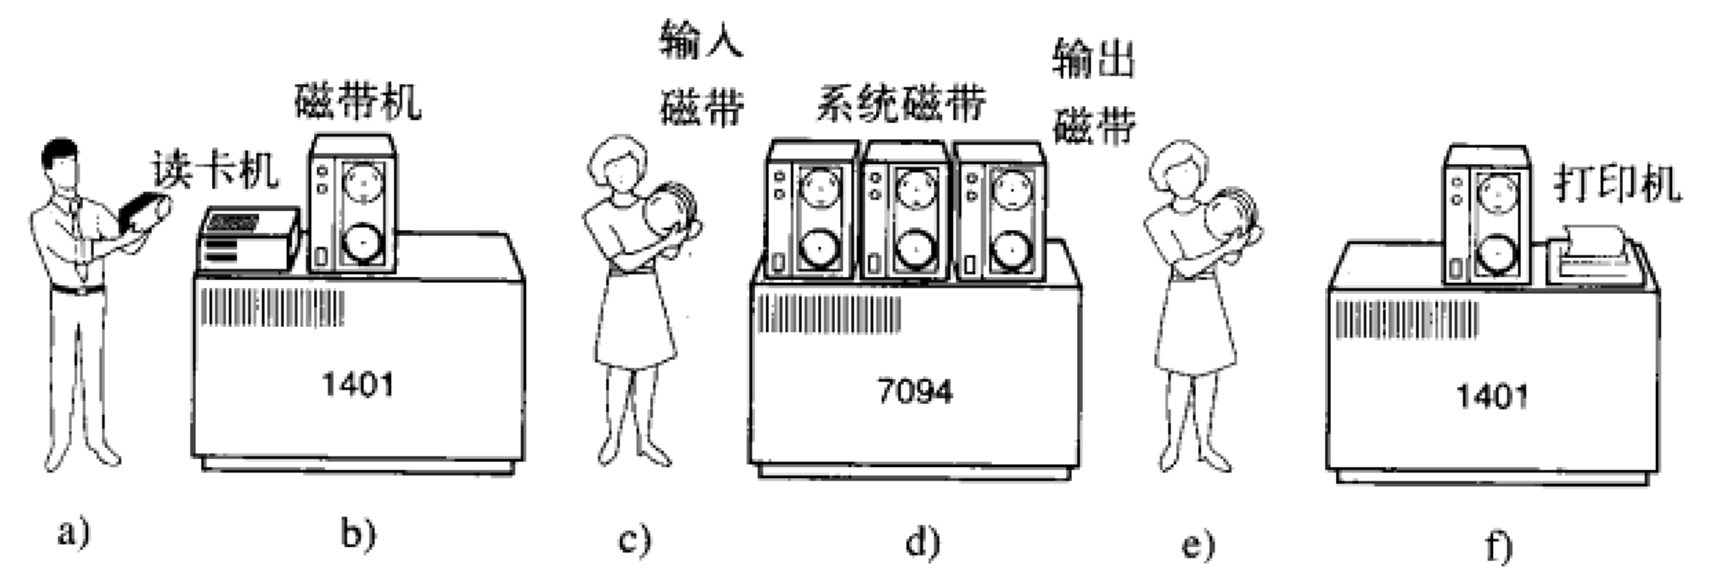
\includegraphics[width=.8\textwidth]{../Fig/btss.png}
  \caption{批处理系统}
  \label{fig:btss}
\end{figure}

\begin{description}
\item[a.]程序员将打孔纸带拿到1401机\footnote{IBM 1401:数据处理计算机\cite{1401dps}}
\item[b.]1401机将批处理作业读到磁带上
\item[c.]操作员将输入磁带送至7094机\footnote{IBM 7094:专为大型科学计算而设计,具有出色的性价比和扩展的计算能力\cite{7094dps}}
\item[d.]7094机进行计算
\item[e.]操作员将输出磁带送到1401机
\item[f.]1401机打印输出
\end{description}

在这里,操作系统的工作已经由完全的人工转换到一部分人工操作交由机器完成,工作效率较之前大大提高,
并且,由于加入了磁带,计算机完成的工作也将及时得到保存。
操作系统的工作已经开始有一定的流程化了。

% -------------

\subsection{第三代:集成电路}

采用集成电路的第三代计算机较分立晶体管的第二代计算机在性能/价格比上有了很大的提高,
第三代操作系统加入了多道程序设计和分时系统,可以适应多道程序同时运行的任务。
\begin{enumerate}
  \item 多道程序设计主要目的是解决CPU因等待磁带或其他I/O操作而暂停工作,多道程序设计可以使CPU在程序a的I/O操作时运行程序b\cite{tanenbaum2009modern}。
  \item 分时系统解决的主要问题是多用户使用分离的终端,却操作同一台计算机。
\end{enumerate}

% -------------

\subsection{第四代:个人计算机}

大规模集成电路进一步减小了计算机的大小,进一步为计算机进入大众视野做好了铺垫。
现在使用的台式机和笔记本就是属于第四代计算机发展的较高版本。

第四代计算机和之前的计算机比较而言在于同一台终端的使用人数,
第四代之前的计算机主要用于科研和大规模计算,所有硬件都是为这些作业而工作,操作系统也只用为这些作业安排调度,
而每个人都能拥有自己的计算机,那么计算机就需要有更多个性化的东西,这对操作系统提出了更多的要求:

\begin{enumerate}
  \item 更多的进程
  \item 更大的存储空间(文件管理)
  \item 更多设备接入(如鼠标)
  \item 网络要求的实现
  \item 对外防护的要求
  \item 对外提供接口(图形化显示)
\end{enumerate}

% -------------

\subsection{第五代:移动计算机}

第五代计算机是便携式计算机,也就是智能手机或者智能平板设备,较之第四代计算机最大的不同在于易于携带,
但是缺点也很显著,受到设备体积和电池的限制,性能受到很大的影响。

第五代计算机对操作系统有了新的要求:
\begin{enumerate}
  \item 从待机状态极快的响应
  \item 电量控制(即低成本完成作业)
\end{enumerate}

% ----------

\subsection{小结}

纵观操作系统的发展史,发展的中心问题是“如何更低成本完成更多的任务”,
而发展的关键节点是多道程序设计以及分时系统。

展望计算机的发展史,大胆的推测下一代计算机可能就是"computer everywhwere",
而那时操作系统也会有新的发展。

\section{操作系统的规范化}

\subsection{Unix及类Unix}
Unix 及类 Unix 将用户空间与系统空间划分开,以此规定内核的边界,将存在于系统空间的代码与数据的集合称为内核。
由此也存在了不同的 CPU 运行模式:系统态和用户态。
\begin{enumerate}
  \item 系统调用接口
  \item 进程管理
  \item 内存管理
  \item 虚拟文件系统
  \item 网络堆栈
  \item 设备驱动程序
\end{enumerate}

\subsection{Windows}

Microsoft Windows 与 Unix 最大的不同是,它将较低层的离硬件最近的一部分叫做“内核”,
因此,Windows也将图形界面和视窗机制的实现也放在了内核中。

大体来说,Windows内核层次如下:
\begin{enumerate}
  \item 系统调用接口
  \item 中断/异常入口
  \item Executive (管理层)、对象管理、内存管理、进程管理、安全管理、I/O管理等~\cite{毛德操2005windows}
  \item 核心层、设备驱动底层
  \item HAL(硬件抽象层)
\end{enumerate}

\subsection{小结}
从市场中用户数量较多的两大操作系统平台看,操作系统已经趋于规范化,功能方面也趋于成熟,
两大操作系统的功能都非常完备,但功能多了的坏处就是bug出现的概率也随之变高,
所以windows的蓝屏和linux的系统抖动等操作系统问题都对用户造成了极大的困扰。

想要解决这些问题较好的办法就是精简功能,从降低代码数量开始降低系统bug的出现概率,
精简功能则要很好的处理好必要功能和非必要功能的筛选分类。